%%%%%%%%%%%%%%%%%%%%%%%%%%%%%%%%%%%%%%%%%%%%%%%%%%%%%%%%%%%%%%%%%%% 
%                                                                 %
%                            CHAPTER                              %
%                                                                 %
%%%%%%%%%%%%%%%%%%%%%%%%%%%%%%%%%%%%%%%%%%%%%%%%%%%%%%%%%%%%%%%%%%% 

\chapter{Methods for DNA sequence alignment}
\label{ch:algoverzicht}


\section{DNA sequence aligning}

The human genome (e.g. $hg19$) is used as a reference genome for all sequenced human DNA. However, the genetic code of all humans is slightly different, which also holds true for all other organisms. Genetic sequence alignment is the science where you try to align 2 sequences with each other so that the amount of differences is minimal. In this chapter, the most frequently used algorithms are discussed.

\subsection{Alignment in general}

In genetic codes, there are 3 types of differences between the given sequence and the reference:

\begin{itemize}
	\item Insertion: one or more bases have been added in the genetic code in a specific spot.
	\item Deletion: one or more bases have been removed from the genetic code in a specific spot.
	\item Substitution: one or more bases have been substituted by other bases.
\end{itemize}

Inserts and deletions are often described by a single term, \emph{indel}.

For example: if we want to align the following sequences:
\begin{lcverbatim}
	Seq1: ATATCGGC
	Seq2: ATCG
\end{lcverbatim}
The alignment itself can now be done in different ways. Possible alignments are:
\begin{lcverbatim}
	Alignment 1
	Seq1: AtaTCgGc
	Seq2: A--TC-G-
	Alignment 2
	Seq1: atATCGgc
	Seq2: --ATCG--
\end{lcverbatim}
Which alignment that is the actual output, depends on the algorithm and the given parameters (penalty and similarity scores). The '-' character represents a base that is not present.

Keep in mind, there is no one "correct" alignment. The core of the alignment algorithms is the same each time, but the parameters of these algorithms are changed depending on the application.

\section{Local versus global alignment}
\label{S:localVSglobalAlignment}

To explain the difference between local and global alignment, we can take a look at the following example:

\begin{lcverbatim}
	The 2 DNA sequences:
	Seq1: TCCCAGTTTGTGTCAGGGGACACGAG
	Seq2: CGCCTCGTTTTCAGCAGTTATGTGCAGATC
	
	Alignment 1 :
	Seq1: -----------tccCAGTT-TGTGTCAGgggacacgag
	Seq2: cgcctcgttttcagCAGTTATGTG-CAGatc-------
	
	Alignment 2 :
	Seq1 : tcCCa-GTTTgt-GtCAGggg-acaC-GA-g
	Seq2 : cgCCtcGTTTtcaG-CAGttatgtgCaGAtc
\end{lcverbatim}

Both alignments are valid but different. The first alignment is \emph{locally aligned}. This means that the similarities are prioritized in the same region, with the similarity as high as possible. On the other hand, the second alignment is \emph{globally aligned}. Here the similarities over the full length of the sequences are used for the alignment. 

In practice, the local alignment is used most often, since it can give you information of 2 sequences that do not have (approximately) the same length.

\section{Commonly used algorithms}

In this section, we will take a look at some algorithms that are used most often for DNA sequence alignment.


The most used algorithms are often categorized in 2 ways: 

\begin{itemize}
	\item local alignment versus global alignments (see \ref{S:localVSglobalAlignment})
	\item dynamic algorithms versus heuristic algorithms: dynamic algorithms are exact but slow and computationally demanding, whereas heuristic algorithms are faster but are approximations and the best alignment is not guaranteed.
\end{itemize}

Hereunder is a schematic view of some algorithms that are used in practice:

\begin{table}[H]
	\begin{tabular}{lllll}
		\cline{1-3}
		\multicolumn{1}{|l|}{}                          & \multicolumn{1}{l|}{\textbf{Dynamic programming}} & \multicolumn{1}{l|}{\textbf{Heuristic programming}} &  &  \\ \cline{1-3}
		\multicolumn{1}{|l|}{\textbf{Local alignment}}  & \multicolumn{1}{c|}{Smith-waterman}               & \multicolumn{1}{c|}{FASTA, BLAST}                   &  &  \\ \cline{1-3}
		\multicolumn{1}{|l|}{\textbf{Global alignment}} & \multicolumn{1}{c|}{Needleman-Wunsch}             & \multicolumn{1}{c|}{X}                              &  &  \\ \cline{1-3}
		&                                                   &                                                     &  & 
	\end{tabular}
	\caption{Classification of DNA alignment algorithms}
\end{table}


Keep in mind, a lot of other claimed "algorithms" (for example BFAST, ...), are accelerated versions of the Smith-Waterman algorithm.

\subsection{Needleman-Wunsch}
Needleman and Wunch proposed a new algorithm for genetic sequence alignment in 1970, now known as the \emph{Needleman-Wunsch} (N-W) algorithm. Since this algorithm is meant for global alignment, which is seldomly used in practice, further discussion of the algorithm will not be done. However, N-W has a lot of similarities with the Smith-Waterman algorithm, discussed in the next section.

\subsection{Smith-Waterman}
\label{expl:SWanalyse}
The \emph{Smith-Waterman} (S-W) algorithm was first proposed by Temple F. Smith and Michael S. Waterman in 1981  %cit
. It is a variation on the N-W algorithm, adapted for local alignment. It is a dynamic programming technique, so an optimal local alignment is guaranteed. \\

The core of the algorithm is a matrix fillup, with data dependencies on the previous cells. Hereunder an analysis of the algorithm:

\begin{enumerate}
	\item Symbols used in the analysis:
	
	Let sequences $A = a_1 a_2 a_3 \dots a_n$ and $B = b_1 b_2 b_3 \dots b_m$ be the sequences that need to be locally aligned. Here $n$ and $m$ are the lengths of the sequences $A$ and $B$
	
	\item Define the parameters: 
	
	\begin{itemize}
		\item Define $s(a,b)$ be the \emph{similarity matrix} (sometimes also called the \emph{substitution matrix}) for the two sequences. It is used for "rewarding" when $a_i = b_j$ and "punishing" when $a_i \neq b_j$.
		
		In the most general way, we define the similarity score as a matrix of values, e.g.:
		
		\begin{table}[H]
			\centering
			\begin{tabular}{|r|r|r|r|r|}
				\hline
				& \textbf{A} & \textbf{C} & \textbf{G} & \textbf{T} \\ \hline
				\textbf{A} & 3          & -3         & -3         & -3         \\ \hline
				\textbf{C} & -3         & 3          & -3         & -3         \\ \hline
				\textbf{G} & -3         & -3         & 3          & -3         \\ \hline
				\textbf{T} & -3         & -3         & -3         & 3          \\ \hline
			\end{tabular}
			
			\caption{\centering Similarity matrix example}
		\end{table}
		
		Often, there are only 2 scores used (equal or not equal). In this case, the similarity matrix can be condensed as follows:
		
		\begin{align*}
		s(a_i,b_j)=
		\begin{cases}
		+3, \quad a_i=b_j     \\
		-3, \quad a_i\neq b_j
		\end{cases}
		\end{align*}
		
		\item Define $d$ as the \emph{gap penalty} which regulates the score for an insertion or a deletion. This parameter can be:
		
		\begin{itemize}
			\item \emph{Linear}: The penalty is constant. So, in this case, it doesn't matter if the previous was also a gap or not.
			\item \emph{Affine}: An affine gap penalty considers gap opening and extension separately. For the sake of simplicity, my further implementation will not include this refinement of the algorithm. The algorithm can be extended to include this affine gap penalty, but this would make the algorithm more complex and we would limit our ability to develop possible accelerations. It is also expected to affect the DNA mapping on a reference genome. However, if we assume the size of the gaps as small, there won't be much difference in result in comparison with the linear penalty score.
		\end{itemize}
		
		
	\end{itemize}
	
	
	\item The initialization: We construct a scoring matrix $H$ with dimensions $(n+1)\times(m+1)$. The first column and first row we initialize with $0$.
	
	For example: if we want to align the sequences A = $TGTTACGG$ and B = $GGTTGACTA$:
	
	\begin{table}[H]
		\centering
		\begin{tabular}{rrrrrrrrrr}
			&                        & T                      & G                      & T                      & T                      & A                      & C                      & G                      & G                      \\ \cline{2-10} 
			\multicolumn{1}{r|}{}  & \multicolumn{1}{r|}{0} & \multicolumn{1}{r|}{0} & \multicolumn{1}{r|}{0} & \multicolumn{1}{r|}{0} & \multicolumn{1}{r|}{0} & \multicolumn{1}{r|}{0} & \multicolumn{1}{r|}{0} & \multicolumn{1}{r|}{0} & \multicolumn{1}{r|}{0} \\ \cline{2-10} 
			\multicolumn{1}{r|}{G} & \multicolumn{1}{r|}{0} & \multicolumn{1}{r|}{}  & \multicolumn{1}{r|}{}  & \multicolumn{1}{r|}{}  & \multicolumn{1}{r|}{}  & \multicolumn{1}{r|}{}  & \multicolumn{1}{r|}{}  & \multicolumn{1}{r|}{}  & \multicolumn{1}{r|}{}  \\ \cline{2-10} 
			\multicolumn{1}{r|}{G} & \multicolumn{1}{r|}{0} & \multicolumn{1}{r|}{}  & \multicolumn{1}{r|}{}  & \multicolumn{1}{r|}{}  & \multicolumn{1}{r|}{}  & \multicolumn{1}{r|}{}  & \multicolumn{1}{r|}{}  & \multicolumn{1}{r|}{}  & \multicolumn{1}{r|}{}  \\ \cline{2-10} 
			\multicolumn{1}{r|}{T} & \multicolumn{1}{r|}{0} & \multicolumn{1}{r|}{}  & \multicolumn{1}{r|}{}  & \multicolumn{1}{r|}{}  & \multicolumn{1}{r|}{}  & \multicolumn{1}{r|}{}  & \multicolumn{1}{r|}{}  & \multicolumn{1}{r|}{}  & \multicolumn{1}{r|}{}  \\ \cline{2-10} 
			\multicolumn{1}{r|}{T} & \multicolumn{1}{r|}{0} & \multicolumn{1}{r|}{}  & \multicolumn{1}{r|}{}  & \multicolumn{1}{r|}{}  & \multicolumn{1}{r|}{}  & \multicolumn{1}{r|}{}  & \multicolumn{1}{r|}{}  & \multicolumn{1}{r|}{}  & \multicolumn{1}{r|}{}  \\ \cline{2-10} 
			\multicolumn{1}{r|}{G} & \multicolumn{1}{r|}{0} & \multicolumn{1}{r|}{}  & \multicolumn{1}{r|}{}  & \multicolumn{1}{r|}{}  & \multicolumn{1}{r|}{}  & \multicolumn{1}{r|}{}  & \multicolumn{1}{r|}{}  & \multicolumn{1}{r|}{}  & \multicolumn{1}{r|}{}  \\ \cline{2-10} 
			\multicolumn{1}{r|}{A} & \multicolumn{1}{r|}{0} & \multicolumn{1}{r|}{}  & \multicolumn{1}{r|}{}  & \multicolumn{1}{r|}{}  & \multicolumn{1}{r|}{}  & \multicolumn{1}{r|}{}  & \multicolumn{1}{r|}{}  & \multicolumn{1}{r|}{}  & \multicolumn{1}{r|}{}  \\ \cline{2-10} 
			\multicolumn{1}{r|}{C} & \multicolumn{1}{r|}{0} & \multicolumn{1}{r|}{}  & \multicolumn{1}{r|}{}  & \multicolumn{1}{r|}{}  & \multicolumn{1}{r|}{}  & \multicolumn{1}{r|}{}  & \multicolumn{1}{r|}{}  & \multicolumn{1}{r|}{}  & \multicolumn{1}{r|}{}  \\ \cline{2-10} 
			\multicolumn{1}{r|}{T} & \multicolumn{1}{r|}{0} & \multicolumn{1}{r|}{}  & \multicolumn{1}{r|}{}  & \multicolumn{1}{r|}{}  & \multicolumn{1}{r|}{}  & \multicolumn{1}{r|}{}  & \multicolumn{1}{r|}{}  & \multicolumn{1}{r|}{}  & \multicolumn{1}{r|}{}  \\ \cline{2-10} 
			\multicolumn{1}{r|}{A} & \multicolumn{1}{r|}{0} & \multicolumn{1}{r|}{}  & \multicolumn{1}{r|}{}  & \multicolumn{1}{r|}{}  & \multicolumn{1}{r|}{}  & \multicolumn{1}{r|}{}  & \multicolumn{1}{r|}{}  & \multicolumn{1}{r|}{}  & \multicolumn{1}{r|}{}  \\ \cline{2-10} 
		\end{tabular}
		\caption{\centering Example of the initialization of the scoring matrix}
	\end{table}
	
	\item Matrix fill in:
	We fill in the matrix using the following formula:
	
	\begin{align*}
	H_{ij}= max
	\begin{cases}
	H_{i-1,j-1} + s(a_i, b_j),\\
	H_{i-1,j} - d,\\
	H_{i,j-1} - d,\\
	0
	\end{cases}
	\end{align*}
	
	If we keep in mind that the value of a cell may never be lower than 0, we can represent the data dependencies in the following schematic:
	
	
	\begin{figure}[H]
		\centering
		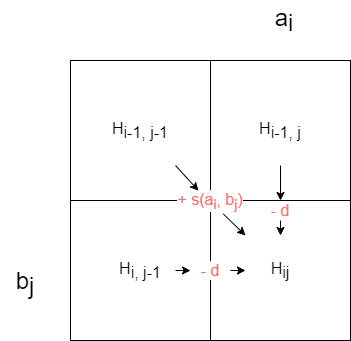
\includegraphics[width=0.5\textwidth]{ExisMethods/Dependencies_SW.png}
		\caption{Data dependencies in the $H$ matrix}
		\label{fig:DatDep}
	\end{figure}
	
	Where $s(a,b)$ and $d$ are the parameters of the algorithm. If we use the following values as an example:
	
	\begin{align*}
	s(a_i,b_j)=
	\begin{cases}
	+3, \quad a_i=b_j     \\
	-3, \quad a_i\neq b_j
	\end{cases} \qquad \text{and} \qquad d = 2
	\end{align*}
	
	We can now fill up the scoring matrix $H$:
	
	\begin{table}[H]
		\centering
		\begin{tabular}{rrrrrrrrrr}
			&                        & T                      & G                      & T                      & T                      & A                       & C                       & G                       & G                      \\ \cline{2-10} 
			\multicolumn{1}{r|}{}  & \multicolumn{1}{r|}{0} & \multicolumn{1}{r|}{0} & \multicolumn{1}{r|}{0} & \multicolumn{1}{r|}{0} & \multicolumn{1}{r|}{0} & \multicolumn{1}{r|}{0}  & \multicolumn{1}{r|}{0}  & \multicolumn{1}{r|}{0}  & \multicolumn{1}{r|}{0} \\ \cline{2-10} 
			\multicolumn{1}{r|}{G} & \multicolumn{1}{r|}{0} & \multicolumn{1}{r|}{0} & \multicolumn{1}{r|}{3} & \multicolumn{1}{r|}{1} & \multicolumn{1}{r|}{0} & \multicolumn{1}{r|}{0}  & \multicolumn{1}{r|}{0}  & \multicolumn{1}{r|}{3}  & \multicolumn{1}{r|}{3} \\ \cline{2-10} 
			\multicolumn{1}{r|}{G} & \multicolumn{1}{r|}{0} & \multicolumn{1}{r|}{0} & \multicolumn{1}{r|}{3} & \multicolumn{1}{r|}{1} & \multicolumn{1}{r|}{0} & \multicolumn{1}{r|}{0}  & \multicolumn{1}{r|}{0}  & \multicolumn{1}{r|}{3}  & \multicolumn{1}{r|}{6} \\ \cline{2-10} 
			\multicolumn{1}{r|}{T} & \multicolumn{1}{r|}{0} & \multicolumn{1}{r|}{3} & \multicolumn{1}{r|}{1} & \multicolumn{1}{r|}{6} & \multicolumn{1}{r|}{4} & \multicolumn{1}{r|}{2}  & \multicolumn{1}{r|}{0}  & \multicolumn{1}{r|}{1}  & \multicolumn{1}{r|}{4} \\ \cline{2-10} 
			\multicolumn{1}{r|}{T} & \multicolumn{1}{r|}{0} & \multicolumn{1}{r|}{3} & \multicolumn{1}{r|}{1} & \multicolumn{1}{r|}{4} & \multicolumn{1}{r|}{9} & \multicolumn{1}{r|}{7}  & \multicolumn{1}{r|}{5}  & \multicolumn{1}{r|}{3}  & \multicolumn{1}{r|}{2} \\ \cline{2-10} 
			\multicolumn{1}{r|}{G} & \multicolumn{1}{r|}{0} & \multicolumn{1}{r|}{1} & \multicolumn{1}{r|}{6} & \multicolumn{1}{r|}{4} & \multicolumn{1}{r|}{7} & \multicolumn{1}{r|}{6}  & \multicolumn{1}{r|}{4}  & \multicolumn{1}{r|}{8}  & \multicolumn{1}{r|}{6} \\ \cline{2-10} 
			\multicolumn{1}{r|}{A} & \multicolumn{1}{r|}{0} & \multicolumn{1}{r|}{0} & \multicolumn{1}{r|}{4} & \multicolumn{1}{r|}{3} & \multicolumn{1}{r|}{5} & \multicolumn{1}{r|}{10} & \multicolumn{1}{r|}{8}  & \multicolumn{1}{r|}{6}  & \multicolumn{1}{r|}{5} \\ \cline{2-10} 
			\multicolumn{1}{r|}{C} & \multicolumn{1}{r|}{0} & \multicolumn{1}{r|}{0} & \multicolumn{1}{r|}{2} & \multicolumn{1}{r|}{1} & \multicolumn{1}{r|}{3} & \multicolumn{1}{r|}{8}  & \multicolumn{1}{r|}{13} & \multicolumn{1}{r|}{11} & \multicolumn{1}{r|}{9} \\ \cline{2-10} 
			\multicolumn{1}{r|}{T} & \multicolumn{1}{r|}{0} & \multicolumn{1}{r|}{3} & \multicolumn{1}{r|}{1} & \multicolumn{1}{r|}{5} & \multicolumn{1}{r|}{4} & \multicolumn{1}{r|}{6}  & \multicolumn{1}{r|}{11} & \multicolumn{1}{r|}{10} & \multicolumn{1}{r|}{8} \\ \cline{2-10} 
			\multicolumn{1}{r|}{A} & \multicolumn{1}{r|}{0} & \multicolumn{1}{r|}{1} & \multicolumn{1}{r|}{0} & \multicolumn{1}{r|}{3} & \multicolumn{1}{r|}{2} & \multicolumn{1}{r|}{7}  & \multicolumn{1}{r|}{9}  & \multicolumn{1}{r|}{8}  & \multicolumn{1}{r|}{7} \\ \cline{2-10} 
		\end{tabular}
		\caption{\centering Example of a populated scoring matrix}
	\end{table}
	
	
	\item Traceback: We start at the cell with the highest score in the matrix $H$. Starting here we only move left, up or diagonally (left-up) to the cell on which the value in the cell was based until we hit a cell with value $0$.
	
	
	\begin{table}[H]
		\centering
		\begin{tabular}{rrrrrrrrrr}
			&                        & T                                              & G                                              & T                                              & T                                              & A                                               & C                                               & G                       & G                      \\ \cline{2-10} 
			\multicolumn{1}{r|}{}  & \multicolumn{1}{r|}{0} & \multicolumn{1}{r|}{0}                         & \multicolumn{1}{r|}{0}                         & \multicolumn{1}{r|}{0}                         & \multicolumn{1}{r|}{0}                         & \multicolumn{1}{r|}{0}                          & \multicolumn{1}{r|}{0}                          & \multicolumn{1}{r|}{0}  & \multicolumn{1}{r|}{0} \\ \cline{2-10} 
			\multicolumn{1}{r|}{G} & \multicolumn{1}{r|}{0} & \multicolumn{1}{r|}{\cellcolor[HTML]{FFCCC9}0} & \multicolumn{1}{r|}{3}                         & \multicolumn{1}{r|}{1}                         & \multicolumn{1}{r|}{0}                         & \multicolumn{1}{r|}{0}                          & \multicolumn{1}{r|}{0}                          & \multicolumn{1}{r|}{3}  & \multicolumn{1}{r|}{3} \\ \cline{2-10} 
			\multicolumn{1}{r|}{G} & \multicolumn{1}{r|}{0} & \multicolumn{1}{r|}{0}                         & \multicolumn{1}{r|}{\cellcolor[HTML]{DAE8FC}3} & \multicolumn{1}{r|}{1}                         & \multicolumn{1}{r|}{0}                         & \multicolumn{1}{r|}{0}                          & \multicolumn{1}{r|}{0}                          & \multicolumn{1}{r|}{3}  & \multicolumn{1}{r|}{6} \\ \cline{2-10} 
			\multicolumn{1}{r|}{T} & \multicolumn{1}{r|}{0} & \multicolumn{1}{r|}{3}                         & \multicolumn{1}{r|}{1}                         & \multicolumn{1}{r|}{\cellcolor[HTML]{DAE8FC}6} & \multicolumn{1}{r|}{4}                         & \multicolumn{1}{r|}{2}                          & \multicolumn{1}{r|}{0}                          & \multicolumn{1}{r|}{1}  & \multicolumn{1}{r|}{4} \\ \cline{2-10} 
			\multicolumn{1}{r|}{T} & \multicolumn{1}{r|}{0} & \multicolumn{1}{r|}{3}                         & \multicolumn{1}{r|}{1}                         & \multicolumn{1}{r|}{4}                         & \multicolumn{1}{r|}{\cellcolor[HTML]{DAE8FC}9} & \multicolumn{1}{r|}{7}                          & \multicolumn{1}{r|}{5}                          & \multicolumn{1}{r|}{3}  & \multicolumn{1}{r|}{2} \\ \cline{2-10} 
			\multicolumn{1}{r|}{G} & \multicolumn{1}{r|}{0} & \multicolumn{1}{r|}{1}                         & \multicolumn{1}{r|}{6}                         & \multicolumn{1}{r|}{4}                         & \multicolumn{1}{r|}{\cellcolor[HTML]{DAE8FC}7} & \multicolumn{1}{r|}{6}                          & \multicolumn{1}{r|}{4}                          & \multicolumn{1}{r|}{8}  & \multicolumn{1}{r|}{6} \\ \cline{2-10} 
			\multicolumn{1}{r|}{A} & \multicolumn{1}{r|}{0} & \multicolumn{1}{r|}{0}                         & \multicolumn{1}{r|}{4}                         & \multicolumn{1}{r|}{3}                         & \multicolumn{1}{r|}{5}                         & \multicolumn{1}{r|}{\cellcolor[HTML]{DAE8FC}10} & \multicolumn{1}{r|}{8}                          & \multicolumn{1}{r|}{6}  & \multicolumn{1}{r|}{5} \\ \cline{2-10} 
			\multicolumn{1}{r|}{C} & \multicolumn{1}{r|}{0} & \multicolumn{1}{r|}{0}                         & \multicolumn{1}{r|}{2}                         & \multicolumn{1}{r|}{1}                         & \multicolumn{1}{r|}{3}                         & \multicolumn{1}{r|}{8}                          & \multicolumn{1}{r|}{\cellcolor[HTML]{34CDF9}13} & \multicolumn{1}{r|}{11} & \multicolumn{1}{r|}{9} \\ \cline{2-10} 
			\multicolumn{1}{r|}{T} & \multicolumn{1}{r|}{0} & \multicolumn{1}{r|}{3}                         & \multicolumn{1}{r|}{1}                         & \multicolumn{1}{r|}{5}                         & \multicolumn{1}{r|}{4}                         & \multicolumn{1}{r|}{6}                          & \multicolumn{1}{r|}{11}                         & \multicolumn{1}{r|}{10} & \multicolumn{1}{r|}{8} \\ \cline{2-10} 
			\multicolumn{1}{r|}{A} & \multicolumn{1}{r|}{0} & \multicolumn{1}{r|}{1}                         & \multicolumn{1}{r|}{0}                         & \multicolumn{1}{r|}{3}                         & \multicolumn{1}{r|}{2}                         & \multicolumn{1}{r|}{7}                          & \multicolumn{1}{r|}{9}                          & \multicolumn{1}{r|}{8}  & \multicolumn{1}{r|}{7} \\ \cline{2-10} 
		\end{tabular}
		\caption{\centering Example of a traceback in S-W}
	\end{table}
	
	From this traceback we can now deduce the following alignment:
	
	\begin{lcverbatim}
		GTT-AC
		||||||
		GTTGAC
	\end{lcverbatim}
	
	This alignment is the output of our algorithm.
	
\end{enumerate}

\section{Problem definition}

\subsection{Mapping to a reference genome}

From the DNA sequencing machines, we get a big amount of reads in the FASTQ format. We should note that all these reads are worthless without a proper interpretation.

In most cases, the first step in the analysis of the reads is knowing from which part of the genome it's derived. Typically, the read is compared with the whole genome in a local alignment, for example with the Smith-Waterman algorithm. As an output, we would get the position in the human genome and an alignment with its score (how well the sequence fits in that spot). This practice is commonly referred to as \emph{Mapping to reference genome}.

Since the reads from DNA sequencing machines are 75 to 300 bases long, and the whole human genome is approximately 3 billion bases, this comparison is computationally a very intensive task. If we analyze the S-W algorithm (as we have done in \ref{expl:SWanalyse}), we can see that the value of each cell in the matrix is only dependent on the left-upmost 3 cells. Therefore, It leads us to believe that this algorithm can be accelerated on other hardware solutions such as an FPGA (which will be discussed in chapter \ref{ch:Platforms}) since S-W is heavily parallelizable.

In most clinical applications where mapping to a human reference genome is used, the number of reads to be compared with the genome is in the millions.

\begin{figure}[H]
	\centering
	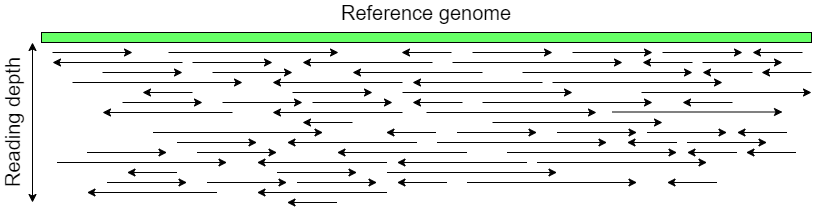
\includegraphics[width=0.95\textwidth]{problemDefinition/MappingRefGen.png}
	\caption{Mapping to a reference genome. The direction of the read is represented by arrows}
	\label{fig:mapRefGen}
\end{figure}

Since the read can be from the complementary DNA molecule in the double helix, the sequences can be in forward $[5' \rightarrow 3']$ direction, or in complementary $[3' \rightarrow 5']$ direction. To transform that read to the used reference genome direction we need to perform the following changes to the read to make its reverse complementary:
\begin{enumerate}
	\item The bases should be changed to their corresponding base in the base pair;
	\item The sequence should be reversed.
\end{enumerate}
We have no way of knowing in which direction the read is taken, both the forward and the backward possibility should be compared with the reference and the best-aligned version of these two should be chosen.

Please note, in most normal cases we can assume the distribution of reads is practically uniform. Therefore, each base in the human genome will be covered by a statistically expected amount of reads. This amount is referred to as the \emph{reading depth}.


\subsection{The sam and bam file format}
\label{expl:SAM}

As a convention, the output of mapping algorithms is in a \emph{SAM} (Sequence Alignment Map) or \emph{BAM} (Binary Alignment Map) file format. The BAM file format is just a compressed version of the SAM format, but the SAM format is more readable, which makes it easier for troubleshooting. There exist a lot of tools to transform a SAM to BAM file already, so in this thesis, we will focus on the SAM format. A SAM file consists of two sections: a header and an alignment section. 

%src:http://samtools.github.io/hts-specs/SAMv1.pdf

\subsubsection{Header}
The header is used for information that is independent of the alignments, such as the name of the used algorithm, reference genome, used commands during generation, etc.
The header must be at the beginning of the file, before the alignment section. Each line of the header field must start with an '@' character, so these lines are easily distinguished from lines the alignment section.

\subsubsection{Alignment Section}
Each line in the alignment section represents one mapped sequence and consists of 11 mandatory and some optional fields, which are separated with a tab.

The 11 mandatory fields are:
\begin{enumerate}
	
	\item \textbf{Qname}: this is the name of the query (the sequence to match) and can be found on the first line of the FASTQ file, which is the input to the mapping algorithm.
	
	\item \textbf{FLAG}: a combination of bitwise flags where each bit has a specific interpretation. It consists of 11 bits, but for basic alignments only 2 fields are important:
	\begin{itemize}
		\item bit 2 (binary: $00000000X00$, integer value 4) is set to $1$ if the sequence is unmapped or the map is not found
		\item bit 4 (binary: $000000X0000$, integer value 16) is set to $1$ if the sequence has been mapped as its reverse complement.
	\end{itemize}
	
	\item \textbf{Rname}: the name of the reference genome. This can be found on the first line of the FASTA file, where the reference genome is stored. If the read is unmapped, this field contains a '*' character
	
	\item \textbf{Pos}: the position of the leftmost base in the alignment. Keep in mind that the indexing of the reference starts with 1 for the first base.
	
	\item \textbf{MapQ}: the mapping quality, which indicates how good the sequence fits in the specific position. This can be any value between 0 and 254. Value 255 is a reserved value to represent an unavailable quality.
	
	\item \textbf{CIGAR}, which stands for \textit{Concise Idiosyncratic Gapped Alignment Report}. It is a string that indicates where the matches (M), insertions (I), and deletions (D) occur. For example, if the CIGAR states $3M1I6M2D10M$ this means from left to right: 3 matches, then an insertion, followed by 6 matches, 2 deletions, and finally 10 matches. In case the sequence is unmapped, this field should be filled with a '*' character
	
	\item \textbf{Rnext}: reference sequence name of the primary alignment of the text read in the template. For this thesis, we will fill this field with a '*' character. 
	
	\item \textbf{Pnext}: the position of the primary alignment of the next read in the template. For this thesis, we will fill this field with a '0' character.
	
	\item \textbf{Tlen}: the observed template length, from the first till last mapped base. For this thesis, we will fill this field with a '0' character.
	
	\item \textbf{Seq}: the full sequence. This can be found in the FASTQ file on the second line.
	
	\item \textbf{Qual}: the qualities of the sequence, also given by the FASTQ file on the fourth line.
	
\end{enumerate}

An example of one line in a SAM file:
\begin{lcverbatim}
	SRR11   0   MN98   25   254   7M   0   0   GTTAAAG   BBBBBCB
\end{lcverbatim}
In this example:
\begin{itemize}
	\item The name of the sequence is $SRR11$
	\item The read is matched in the $[5' -> 3']$ direction
	\item The match is found at the 25th base of the reference genome
	\item The mapping quality is 254
	\item CIGAR = $7M$, so a perfect match
	\item The sequence is $GTTAAAG$ with quality $BBBBBCB$
\end{itemize}

\subsection{Clinical application}

In virtually all sequencing applications DNA alignment and reference mapping is needed. Applications which involve whole genome sequencing are particullarly hampered by a long computational analysis time.

We will discuss as examples two clinical applications of mapping to a reference genome.

\begin{enumerate}
	\item \textbf{\emph{NIPT} (non-invasive prenatal testing), a test for detecting genetic defects in a foetus.}\newline
	During or after conception, DNA can be lost or gained in the fertilized egg cell. This can result in a severe syndrome of the child. For example, Down syndrome is caused by a trisomy of chromosome 21. Normally all chromosomes are present twice in each cell, one from the mother and the other from the father. In Down syndrome patients something went wrong during cell division at the very early stage of development, and the fetus has in its cells three times chromosome 21. 
	Because chromosome 21 is quite small and does not contain that many genes, the child can survive, though with typical mental and clinical problems.
	
	\begin{figure}[H]
		%src: http://www.anatomybox.com/wp-content/uploads/2011/07/Trisomy-21-male.png
		\centering
		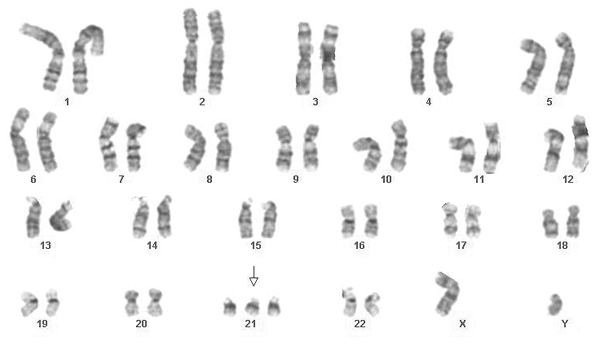
\includegraphics[width=0.5\textwidth]{clinicalAppl/trisomy-21.png}
		\caption{Trisomy 21 karyotype. The trisomy of chromosome-21 is indicated by an arrow}
		\label{fig:tri21}
	\end{figure}
	
	
	Before high throughput DNA sequencing technologies were available like they are today, testing if a fetus has a trisomy-21 could only be done by taking a small amount of amniotic fluid (fluid around the fetus). However, to obtain this fluid there was a need for a risky invasive procedure (called \emph{amniocentesis}) leading sometimes to termination of the pregnancy.
	
	It is known that small amounts of DNA of the fetus are present in the blood of the mother, in the cell-free DNA (\emph{cfDNA}) which we find in the blood plasma (the clear, aqueous part of the blood). The blood plasma is used by our body to transport 'waste', including DNA from cells that were broken down. When fetal cells die, which is a normal process, the building blocks of these cells are transported in the plasma of the blood from the mother, included small DNA fragments from the fetus.
	
	\emph{NIPT} (non-invasive prenatal testing) is used to analyze DNA derived from the mother's blood. A large number of short cfDNA fragments are sequenced at random.  Then, each sequence is mapped to the whole human genome to find out where it comes from. Finally, the distribution of these reads is calculated. If we observe a higher frequency of reads as compared to normal individuals coming from chromosome-21, it is almost certain that the fetus has Down's syndrome.
	
	\begin{figure}[H]
		%src: https://mail.google.com/mail/u/0/#search/nipt/FMfcgxwHMsQcgsbNLGvDkDqXLjxnNdWR?projector=1&messagePartId=0.1
		\centering
		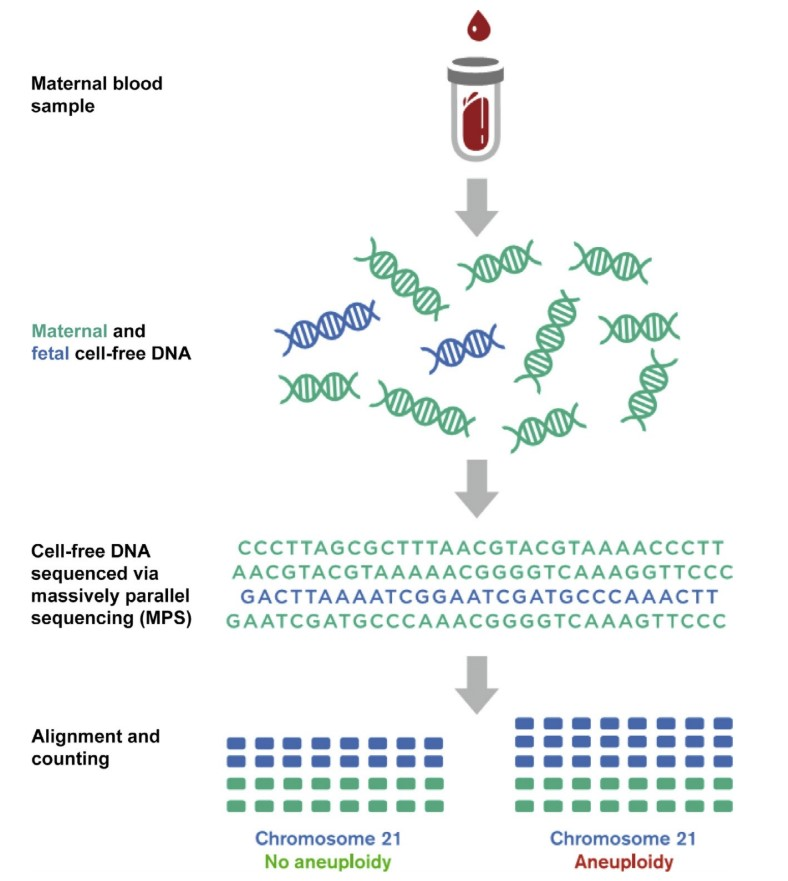
\includegraphics[width=0.5\textwidth]{clinicalAppl/NIPTkadering.jpg}
		\caption{A schematic overview of the NIPT test}
		\label{fig:NIPT}
	\end{figure}
	
	Using the same method, we can also find other defects in the number of chromosomes. For example trisomy 18 (Edwards syndrome), trisomy 13 (Patau syndrome), or even in the sex chromosomes, such as XXY (Klinefelter syndrome) or lack of a second X or a Y chromosome (Turner syndrome).
	
	\item \textbf{Shallow whole-genome sequencing of tumor DNA.}\newline
	It is a known fact that damaged DNA can lead to tumor development. This damage can be single bases changes but can also be loss or gain of large DNA sequences where important genes are located. When someone is diagnosed with cancer, the knowledge of which DNA regions are lost or gained can be important to decide on treatment. 
	
	A relatively new technique to detect all gains and losses of DNA material in one single experiment is shallow whole-genome sequencing. The technique is performed as follows: DNA from the tumor is fragmented (it is broken in small pieces, eg. by a fragmentase enzyme or by high-frequency sound). These pieces are sequenced randomly, and with a mapping algorithm to the reference genome, the over- or underrepresentation of reads (as compared with a normal sample) indicates if regions of the DNA have changed, and which regions these are.
\end{enumerate}